\chapter{Potencial eléctrico }
Cuando una partícula con carga se mueve en un campo eléctrico, el campo ejerce una fuerza que efectúa \textit{trabajo} sobre la partícula. Este trabajo siempre se puede expresar en términos de la energía potencial eléctrica\footnote{O simplemente \textit{potencial eléctrico} o \textit{potencial}}. Una diferencia de potencial entre un punto y otro reciba el nombre de \textit{voltaje}.

\section{Energía potencial eléctrica}
Cuando una fuerza $\vec{F}$ actúa sobre una partícula que se mueve de un punto $a$ a un punto $b$, el trabajo $W_{a\to b}$ efectuado por la fuerza está dado por la siguiente \textit{integral de línea}:

\begin{equation}\label{23.1}\marginnote{Trabajo realizado por una fuerza}
W_{a\to b}=\int_a^b\vec{F}\cdot d\vec{l}=\int_a^bF\cos\phi dl
\end{equation}

donde $d\vec{l}$ es un desplazamiento infinitisimal a lo largo de la trayectoria de la partícula, y $\phi$ es el ángulo entre $\vec{F}$ y $d\vec{l}$ 	en cada punto de la trayectoria.

Si la fuerza $\vec{F}$ es \textit{conservativa}, el trabajo realizado por esta siempre se puedo expresar en términos de una \textbf{energía potencial} $U$. Cuando la partícula se mueve de un punto donde la energía potencial es $U_a$ a otro donde es $U_b$, el cambio de energía potencial es $\Delta U=U_b-U_a$, y el trabajo $W_{a\to b}$ que realiza la fuerza es

\begin{equation}\label{23.2}\marginnote{Trabajo efectuado por una fuerza conservativa}
\boxed{W_{a\to b}=U_a-U_b=-(U_b-U_a)=-\Delta U}
\end{equation}

En tercer lugar, el teorema del trabajo y la energía establece que el cambio en la energía cinética $\Delta K=K_b+K_a$ durante cualquier desplazamiento es igual al trabajo \textit{total} realizado sobre la partícula. Si el único trabajo efectuado sobre la partícula lo realizan fuerzas conservativas, entonces la ecuación \ref{23.2} da el trabajo total, y $K_b-K_a=-(U_b-U_a)$. Es decir, 

\begin{equation}\label{23.3}
K_a+U_a=K_b+U_b
\end{equation}

Es decir, en estas circunstancias, la energía mecánica total (cinética más potencial) se
\textit{conserva}.

\subsection{Energía potencial eléctrica de un campo uniforme}
\begin{figure}[h]
\centering
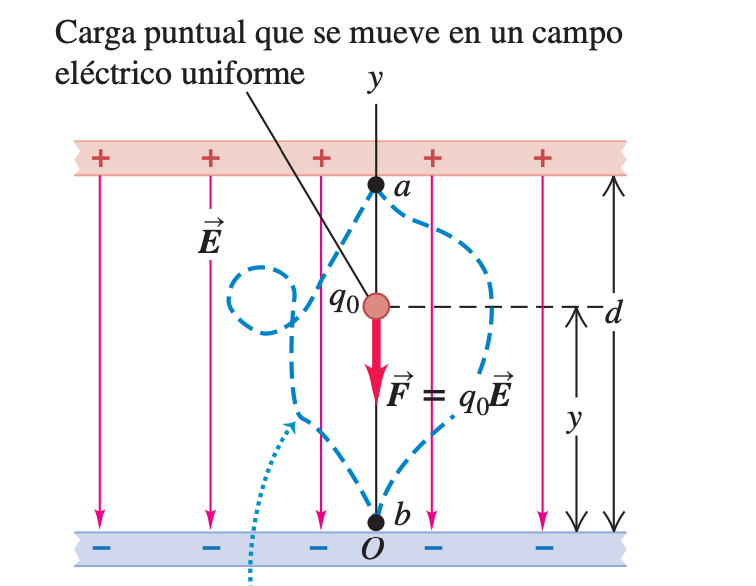
\includegraphics[scale=0.5]{fig/energia_potencial}
\caption{Trabajo realizado sobre una carga puntual que se mueve en un campo eléctrico uniforme. El trabajo realizado por la fuerza eléctrica es el mismo para cualquier trayectoria de $a$ a $b$: $W_{a\to b}=-\Delta U=q_0Ed$} 
\label{fig:energia_potencial}
\end{figure}

En la figura \ref{fig:energia_potencial} un par de placas metálicas paralelas con carga generan un campo eléctrico uniforme descendente y con magnitud $E$. El campo ejerce una fuerza hacia abajo con magnitud $F=q_0E$ sobre una carga de prueba positiva $q_0$. A medida que la carga se mueve hacia abajo una distancia $d$ del punto $a$ al punto $b$, la fuerza sobre la carga de prueba es constante e independiente de su localización. Por lo tanto, el trabajo realizado por el campo eléctrico es 

\begin{equation}\label{23.4}
W_{a\to b}=Fd=q_0Ed
\end{equation}

Este trabajo es positivo, toda vez que la fuerza está en la misma dirección que el desplazamiento neto de la carga de prueba. Este trabajo puede representarse con una función de \textbf{energía potencial} $U$, que para la fuerza eléctrica está dada por

\begin{equation}\label{23.5}
U=q_0Ey
\end{equation}

Cuando la carga de prueba se mueve de la altura $y_a$ a la altura $y_b$, el trabajo realizado sobre la carga por el campo está dado por

\begin{equation}\label{23.6}
W_{a\to b}=-\Delta U=-(U_b-U_a)=-(q_0Ey_b-q_0Ey_a)=q_0E(y_a-y_b)
\end{equation}

\subsection{Energía potencial entre dos cargas puntuales}
El concepto de energía potencial se puede aplicar a una carga puntual en \textit{cualquier} campo eléctrico generado por una distribución de carga estática. 
Cualquier distribución de carga se representa como un conjunto de cargas puntuales. Por consiguiente, es útil calcular el trabajo realizado sobre una carga de prueba $q_0$ que se mueve en el campo eléctrico ocasionado por una sola carga puntual estacionaria $q$.

En primer lugar se considerará un desplazamiento a lo largo de una línea radial, del punto $a$ al punto $b$. La fuerza sobre $q_0$ está dada por la ley de Coulomb, y su componente radial es

\begin{equation}\label{23.7}
F_r=\frac{1}{4\pi\epsilon_0}\frac{qq_0}{r^2}
\end{equation}

Si $q$ y $q_0$ tienen el mismo signo, la fuerza es de repulsión y $F_r$ es positiva; en caso contrario la fuerza es de atracción y $F_r$ es negativa. La fuerza \textit{no} es constante durante el desplazamiento, y se tiene que integrar para obtener el trabajo $W_{a\to b}$ que realiza esta fuerza sobre $q_0$ a medida que $q_0$ se mueve de $a$ a $b$

\begin{equation}\label{23.8}
W_{a\to b}=\int_{r_a}^{r_b}F_rdr=\int_{r_a}^{r_b}\frac{1}{4\pi\epsilon_0}\frac{qq_0}{r^2}dr=\frac{qq_0}{4\pi\epsilon_0}\left(\frac{1}{r_a}-\frac{1}{r_b}\right)
\end{equation}

El trabajo es el mismo para todas las trayectorias posibles entre $a$ y $b$. La fuerza sobre $q_0$ es \textit{conservativa}.\\
Se ve que las ecuaciones \ref{23.2} y \ref{23.8} son cosistentes si se define $qq_0/4\pi\epsilon_0r_a$ como la energia potencial $U_a$ cuando $q_0$ está en el punto $a$, a una distancia $r_a$ de $q$, y se define $qq_0/4\pi\epsilon_0r_b$ como la energía potencial $U_b$ cuando $q_0$ está en el punto $b$, a una distancia $r_b$ de $q$. De esta forma, la energía potencial $U$ cuando la carga de prueba $q_0$ está a cualquier distancia $r$ de la carga $q$ es

\begin{equation}\label{23.9.e_potencial}\marginnote{E. potencial eléctrica de dos cargas $q$ y $q_0$}
\boxed{U=\frac{1}{4\pi\epsilon_0}\frac{qq_0}{r}}
\end{equation}

\textbf{Obervación:} De las ecuaciones \ref{23.9.e_potencial} y \ref{23.7} notamos que tienen similitud. La energía potencial $U$ es proporcional a $1/r$, mientras que la componente de la fuerza $F_r$ es proporcional a $1/r^2$.\\
La energía potencial siempre se define en relación con algún punto de referencia donde $U=0$. En la ecuación \ref{23.9.e_potencial}, $U$ es igual a cero cuando $q$ y $q_0$ están infinitamente alejadas y $r=\infty$. Por lo tanto, \textbf{$U$ representa el trabajo que realizaría el campo de $q$ sobre la carga de prueba $q_0$ si esta última se desplazara de una distancia inicial $r$ al infinito}. La energía potencial $U$ es una propiedad \textit{compartida} de las dos cargas $q$ y $q_0$; es una consecuencia de la \textit{interacción} entre dos cuerpos.

La ley de Gauss dice que el campo eléctrico fuera de cualquier distribución de carga esféricamente simétrica es la misma que habría si toda la carga estuviera en el centro.

\subsection{Energía potencial eléctrica con varias cargas putuales}

\begin{figure}[h]
\centering
\caption{La energía potencial asociada con la carga $q_0$ en el punto a depende de las otras cargas $q_1, q_2$ y $q_3$ y de sus distancias $r_1, r_2$ y $r_3$ desde el punto $a$.}
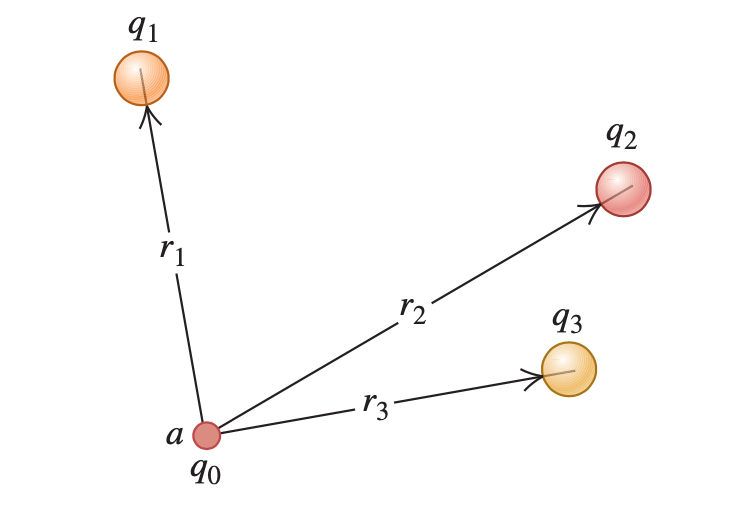
\includegraphics[scale=0.4]{fig/e_potencial_varias}
\label{fig:e_potencial_varias}
\end{figure}

Suponga que el campo eléctrico $\vec{E}$ en el que se desplaza la carga $q_0$ se debe a varias cargas puntuales $q_1, q_2, q_3$, . . . a distancias $r_1, r_2, r_3$, . . . de $q_0$. . El campo eléctrico total en cada punto es la \textit{suma vectorial} de los campos debidos a las cargas individuales, y el trabajo total realizado sobre $q_0$ durante cualquier desplazamiento es la suma de las contribuciones de las cargas individuales. De la ecuación \ref{23.9.e_potencial} se concluye que la energía potencial asociada con la carga de prueba $q_0$ en el punto a en la figura \ref{fig:e_potencial_varias} es la suma \textit{algebraica} (no la suma vectorial).

\begin{equation}\label{23.10}\marginnote{Carga puntual $q_0$ y conjunto de cargas $q_i$}
\boxed{U=\frac{q_0}{4\pi\epsilon_0}\left(\frac{q_1}{r_1}+\frac{q_2}{r_2}+\frac{q_3}{r_3}+\cdots \right)=\frac{q_0}{4\pi\epsilon_0}\sum_{i}\frac{q_i}{r_i}}
\end{equation}

El trabajo efectuado sobre la carga $q_0$ cuando se desplaza de $a$ a $b$ a lo largo de cualquier trayectoria es igual a la diferencia $U_a-U_b$ entre las energías potenciales cuando $q_0$ está en $a$ y en $b$.

Se puede representar \textit{cualquier} distribución de carga como un conjunto de cargas puntuales, por lo que la ecuación \ref{23.10} muestra que \textbf{para todo campo eléctrico debido a una distribución de carga estática, la fuerza ejercida por ese campo es conservativa.}

Las ecuaciones \ref{23.9.e_potencial} y \ref{23.10} definen que $U$ es igual a cero cuando todas las distancias $r_1, r_2, . . .$ son infinitas, es decir, cuando la carga de prueba $q_0$ está muy lejos de todas las cargas que producen el campo.

\subsubsection{Interpretación de la energía potencial eléctrica}
Definimos la energía potencial eléctrica en términos del trabajo realizado por el campo eléctrico sobre una partícula con carga que se mueve en el campo. Cuando una partícula se desplaza del punto $a$ al punto $b$, el trabajo que realiza sobre ella el campo eléctrico es $W_{a\to b}=U_a-U_b$. Por lo tanto, la diferencia de energía potencial $U_a-U_b$ es igual al \textit{trabajo que efectúa la fuerza eléctrica cuando la partícula se desplaza de $a$ a $b$}. Cuando $U_a$ es mayor que $U_b$ el campo realiza trabajo positivo sobre la partícula conforme “cae” de un punto de mayor energía potencial ($a$) a otro con menor energía potencial ($b$).

Un punto de vista alternativo pero equivalente es considerar cuánto trabajo se hubiera tenido que hacer para “subir” la partícula desde un punto $b$, en el que la energía potencial es $U_b$, hasta un punto $a$ en el que la energía potencial tiene un valor mayor $U_a$ (por ejemplo, al empujar dos cargas positivas para acercarlas). Para mover la partícula lentamente (de manera que no se le imparta ninguna energía cinética), es necesario ejercer una fuerza externa adicional $F_{ext}$ que es igual y opuesta a la fuerza del campo eléctrico y realiza un trabajo positivo. La diferencia de energía potencial $U_a-U_b$ se define entonces como el trabajo que debe efectuar una fuerza externa para desplazar la partícula lentamente desde $b$ hasta $a$ en contra de la fuerza eléctrica.

\section{Potencial eléctrico}
El \textbf{potencial} es \textit{la energía potencial por unidad de carga}. Se define el potencial $V$ en cualquier punto en el campo eléctrico como la energía potencial $U$ \textit{por unidad de carga} asociada con una carga de prueba $q_0$ en ese punto:

\begin{equation}\label{23.12}
V=\frac{U}{q_0} \quad\text{o bien, }\quad   U=q_0V
\end{equation}

La unidad del SI para el potencial es el \textbf{volt} (1 V):

\begin{equation*}
1\, \text{V}=1\, \text{J/C}
\end{equation*}

Dividiendo la ecuación \ref{23.2} entre $q_0$:

\begin{equation}\label{23.13}
\frac{W_{a\to b}}{q_0}=-\frac{\Delta U}{q_0}=-\left(\frac{U_b}{q_0}-\frac{U_a}{q_0}\right)=-(V_b-V_a)=V_a-V_b
\end{equation}

$V_a$ y $V_b$ se denominan el \textit{potencial en el punto a} y \textit{potencial en el punto b}, respectivamente. De este modo, el trabajo realizado por unidad de carga por la fuerza eléctrica cuando un cuerpo con carga se desplaza de $a$ a $b$ es igual al potencial en $a$ menos el potencial en $b$.

La diferencia $V_a-V_b$ se llama \textit{potencial de $a$ con respecto a $b$}; en ocasiones esa diferencia se abrevia como $V_{ab}=V_a-V_b$. En los circuitos eléctricos, a diferencia de potencial entre dos puntos con frecuencia se denomina \textbf{voltaje}. Así, la ecuación \ref{23.13} establece: \textbf{$V_{ab}$, el potencial de $a$ con respecto a $b$, es igual al trabajo realizado por la fuerza eléctrica cuando una UNIDAD de carga se desplaza de $a$ a $b$}. Otra interpretación válida tambien es \textbf{$V_{ab}$, el potencial de $a$ con respecto a $b$, es igual al trabajo que debe efectuarse para desplazar con lentitud una UNIDAD de carga de b a a contra la fuerza eléctrica}.

\subsection{Cálculo del potencial eléctrico}
Para encontrar el potencial $V$ debido a una sola carga puntual $q$, se divide la ecuación 	\ref{23.9.e_potencial} entre $q_0$:

\begin{equation}\label{23.14}\marginnote{Potencial debido a una carga puntual}
\boxed{V=\frac{U}{q_0}=\frac{1}{4\pi\epsilon_0}\frac{q}{r}}
\end{equation}

El potencial, como el campo eléctrico, es independiente de la carga de prueba $q_0$ que se utiliza para definirlo.

Para encontrar el potencial debido a un conjunto de cargas puntuales, se divide la ecuación \ref{23.10} entre $q_0$:

\begin{equation}\label{23.15}\marginnote{Potencial debido a un conjunto de cargas puntuales}
\boxed{V=\frac{U}{q_0}=\frac{1}{4\pi\epsilon_0}\sum_i\frac{q_i}{r_i}}
\end{equation}

Cuando se tiene una distribución continua de carga a lo largo de una línea, sobre una superficie o a través de un volumen, se divide la carga en elementos $dq$ y la suma en la ecuación \ref{23.15} se convierte en integral:

\begin{equation}\label{23.16}\marginnote{Potencial debido a un distribución contínua de carga}
\boxed{V=\frac{1}{4\pi\epsilon_0}\int\frac{dq}{r}}
\end{equation}

donde $r$ es la distancia que hay entre el elemento con carga $dq$ y el punto del campo donde se desea obtener $V$

\textbf{Observación}: El \textit{potencial} eléctrico en cierto punto es la energía potencial que estaría asociada a una carga \textit{unitaria} colocada en ese punto. Asimismo, hay que recordar que no tiene que haber una carga en un punto dado para que ahí exista un p tencial $V$.

\subsection{Obtención del potencial eléctrico a partir del campo eléctrico}
La fuerza $\vec{F}$ sobre una carga de prueba $q_0$ se escribe como $\vec{F}=q_0\vec{E}$ por lo que, según la ecuación \ref{23.1}, el trabajo realizado por la fuerza eléctrica conforme la carga de prueba se desplaza de $a$ a $b$ está dado por: 

\begin{equation*}
W_{a\to b}=\int_a^b\vec{F}\cdot d\vec{l}=\int_a^bq_0\vec{E\cdot d\vec{l}}
\end{equation*}

Si se divide entre $q_0$ y se compara el resultado con la ecuación \ref{23.13}, se encuentra que

\begin{equation}\label{23.17}\marginnote{Diferencial de potencial como integral de $\vec{E}$}
\boxed{V_a-V_b=\int_a^b\vec{E}\cdot d\vec{l}=\int_a^bE\cos\phi dl}
\end{equation}

El valor de $V_a-V_b$ es independiente de la trayectoria tomada de $a$ a $b$, del mismo modo en que el valor de $W_{a\to b}$ es independiente de la trayectoria. Para encontrar la ecuación \ref{23.17} hay que recordar que $\vec{E}$ es la fuerza eléctrica por unidad de carga sobre una carga de prueba.

La regla general, válida para \textit{cualquier} campo eléctrico, es la siguiente: desplazarse \textit{en} la dirección de $\vec{E}$ significa hacerlo en la dirección de $V$ \textit{decreciente}, y desplazarse \textit{contra de} la dirección de $\vec{E}$ signifca moverse en la dirección de $\vec{E}$ \textit{creciente}.

Observe que la ecuación \ref{23.17} se puede escribir como 

\begin{equation}\label{23.18}
V_a-V_v=-\int_b^{a}\vec{E}\cdot d\vec{l}
\end{equation}

La ecuación \ref{23.18} se puede interpretar de la siguiente manera: Para mover una unidad de carga lentamente en contra de la fuerza eléctrica, se debe aplicar una fuerza externa por unidad de carga igual a $-\vec{E}$, igual y opuesta a la fuerza eléctrica por unidad de carga $\vec{E}$.

\section{Cálculo del potencial eléctrico}
Cuando se calcula el potencial debido a una distribución de carga, por lo general se sigue una de dos rutas posibles. Si se conoce la distribución de carga se emplea la ecuación \ref{23.15} o la \ref{23.16}. O si se conoce el modo en que el campo eléctrico depende de la posición, se usa la ecuación \ref{23.17} estableciendo que el potencial es igual a cero en algún lugar conveniente.

\section{Superficies equipotenciales}
Una \textbf{superficie equipotencial} es una superficie tridimensional sobre la que el \textit{potencial eléctrico} $V$ es el mismo en todos los puntos. Si una carga de prueba $q_0$ se desplaza de un punto a otro sobre tal superficie, la energía potencial \textit{eléctrica} $q_0V$ permanece constante. Ningún punto puede estar en dos potenciales diferentes, por lo que las superficies equipotenciales para distintos potenciales nunca se tocan o intersecan.

\subsection{Superficies equipotenciales y líneas de campo}
Como la energía potencial no cambia a medida que una carga de prueba se traslada sobre una superficie equipotencial, el campo eléctrico no realiza trabajo sobre esa carga. De ello se deriva que $\vec{E}$ debe ser perpendicular a la superficie en cada punto, de manera que la fuerza eléctrica $q_0\vec{E}$ siempre es perpendicular al desplazamiento de una carga que se mueva sobre la superficie. \textbf{Las líneas de campo y las superficies equipotenciales siempre son perpendiculares entre sí}.

\textbf{Obervación}: En una superficie equipotencial dada, el potencial $V$ tiene el mismo valor en todos los puntos. Sin embargo, en general la magnitud del campo eléctrico $\vec{E}$ \textit{no} es la misma en todos los puntos sobre una superficie equipotencial.

\subsection{Equipotenciales y conductores}
\textbf{Cuando todas las cargas están en reposo, la superficie de un conductor siempre es una superficie equipotencial}. Como el campo eléctrico $\vec{E}$ siempre es perpendicular a una superficie equipotencial, el enunciado se puede demostrar si se prueba que \textbf{cuando todas las cargas están en reposo, el campo eléctrico justo afuera de un conductor debe ser perpendicular a la superficie en cada punto}. Se sabe que $\vec{E}=0$ en todos los lugares del interior del conductor; de otro modo, las cargas se moverían. $\vec{E}$ es perpendicular a la superficie en cada punto.

\section{Gradiente de potencial}
En la ecuación \ref{23.17}, $V_a-V_b$ es el potencial de $a$ con respecto de $b$, es decir, el cambio de potencial encontrado en un despalzamiento de $b$ a $a$. Esto es 

\begin{equation*}
V_a-V_b=\int_b^adV=-\int	_a^bdV
\end{equation*}

donde $dV$ es el cambio infinitesimal del potencial que acompaña un elemento infinitesimal $d\vec{l}$ de la trayectoria de $b$ a $a$. Comparando con la ecuación \ref{23.17} se tiene

\begin{equation*}
-\int_a^bdV=\int_a^b\vec{E}\cdot d\vec{l}
\end{equation*}

Estas dos integrales deben ser iguales para \textit{cualquier} par de límites $a$ y $b$, y para que esto se cumpla los \textit{integrados} deben ser iguales. Por lo tanto, para cualquier desplazamiento infinitesimal $$-dV=\vec{E}\cdot d\vec{l}$$

Las componentes de $\vec{E}$ se relacionan con las derivadas correspondientes de $V$ de la siguiente forma

\begin{equation}\label{23.19}\marginnote{Componentes de $\vec{E}$ en términos de $V$}
\boxed{E_x=-\frac{\partial V}{\partial x} \quad E_y=-\frac{\partial V}{\partial y} \quad E_z=-\frac{\partial V}{\partial z}}
\end{equation}

En términos de vectores unitarios, $\vec{E}$ se escribe como

\begin{equation}\label{23.20}\marginnote{$\vec{E}$ en términos de $V$}
\boxed{\vec{E}=-\left(\hat{i}\frac{\partial V}{\partial x}+\hat{j}\frac{\partial V}{\partial y}+\hat{k}\frac{\partial V}{\partial z}\right)}
\end{equation}

O en forma equivalente

\begin{equation}\label{23.22}
\vec{E}=-\vec{\nabla} V
\end{equation}













































